\section{Grupos e Monoides}
\subsection{As estruturas abstratas}
Se $S$ é um semigrupo de funções, então podemos considerar a função composta como um mapa
\begin{alignat}{2}
  &S \times S \to S \nonumber\\
  &\left(g,f\right)\ \mapsto\ g \circ f.
  \nonumber
\end{alignat}
cujo domínio é o conjunto $S \times S$ dos pares ordenados $(g,f)$ dos elementos de $S$. Estar fechado sob a composição, isto é, $g\in S$ e $f\in S$ implica implica $g\circ f \in S$, garente que $S$ pode servir como o contradomínio do mapa acima.

Lembrando que a função composta é sempre associativa. As propriedades abstratas dos semigrupos de funções são revisadas na definição seguinte.
\begin{definition}[Semigrupos]
  Deixe $S$ ser um conjunto equipado com um mapa
  \begin{alignat}{2}
    &S \times S \to S \nonumber\\
    &\left(x,y\right)\ \mapsto\ g * f
    \nonumber
  \end{alignat}
  associando um elemento $x* y$ de $S$ a cada par ordenado $\left(x,y\right)$ dos elementos de $S$.
  \begin{enumerate}[(a)]
    \item Em geral, o mapa anterior é conhecido como uma operação binária em $S$.
    \item A existência de tal mapa é descrita como o fechamento do conjunto $S$ com respeito a operação *.
    \item O par $\left(S,* \right)$ consistindo do conjunto $S$ com a operação $*$ é chamado de \emph{semigrupo} (ou \emph{semigrupo abstrato}) se a lei associativa $$x * (y * z) = (x * y) * z$$ é válida para todos elementos $x,y$ e $z$ do conjunto $S$.
  \end{enumerate}
\end{definition}

\begin{definition}[Comutatividade]
  Dois elementos $x$ e $y$ de um semigrupo $(S, *)$ são ditos que comutam se $x* y = y* x$. O semigrupo $(S, *)$ é dito ser comutativo se $x* y = y * x$ para todo $x$,$y$ em $S$.
\end{definition}
\begin{exmp}
  Deixe $S$ ser o conjunto ou o intervalo $(1,\infty)$ dos números reais $x$ com $x > 1$. Então $S$ forma um semigrupo sob a multiplicação usual (associativa e comutativa) dos números reais.
\end{exmp}
\begin{exmp}
  Considere o conjunto dos inteiro $\Z$. Então $\Z$ é fechado sob a operação de subtração
  \begin{alignat}{2}
    &\Z \times \Z \to \Z \nonumber\\
    &\left(x,y\right)\ \mapsto\ x - y.
    \nonumber
  \end{alignat}
  No entanto, $\Z$ não forma um semigrupo sob a subtração, pois a subtração não é associativa. De fato, $$3-(5-4)=3-1=2,$$ enquanto $$(3-5)-4=(-2)-4=-6.$$
\end{exmp}

\subsubsection{Monoides}
Um Monoide de funções em um conjunto $X$ é um semigrupo de funções em $X$ que contém a função identidade $id_{X}$ em $X$.
\begin{definition}[Monoides abstratos]
  Deixe $(M, *)$ ser um semigrupo com $*$ como operação. Então $M$ é dito formar um \emph{Monoide} (ou um \emph{Monoide abstrato}) $(M, *, e)$ se ele contém um elemento $e$ satisfazendo $$e * x = x = x * e$$ para todo $x$ em $M$. O elemento $e$ é conhecido como o elemento identidade do Monoide $M$.
\end{definition}
\begin{exmp}
  O semigrupo $S = (1,\infty)$ do exemplo anterior não forma um Monoide. Certamente $S$ não contém o elemento identidade $1$ para a multiplicação dos números reais. De fato, para cada elemento $e$ de $S$, nós temos $e * x > x$ para todo $x$ em $S$. Assim nenhum elemento $e$ (não há nenhum elemento identidade, pois, pela proposição a seguir veremos que o elemento $e$ é único) de $S$ pode satisfazer a definição de Monoide abstrato.
\end{exmp}
\begin{stat}[Unicidade do elemento identidade]
  Deixe $M$ ser um Monoide. Se $e$ e $f$ são elementos identidade de $M$, então $e=f$. Assim o elemento identidade de um Monoide é único.
  \begin{proof}
    Temos $e=e* f = f$. A primeira igualdade é válida pois $f$ é um elemento identidade. A segunda igualdade é válida pois $e$ é um elemento identidade.
  \end{proof}
\end{stat}

\subsubsection{Grupos}
\begin{definition}[Grupos Abstratos]
  Um Monoide $(G,* , e)$ é um \emph{grupo} (ou um \emph{grupo abstrato}) se cada elemento $x$ de $G$ tem um inverso $x^{-1}$ em $G$ com $$x* x^{-1} = e = x^{-1} * x.$$
  Ou seja, um grupo $(G,* , e)$ é um conjunto $G$ com uma multiplicação $*$ satisfazendo as seguintes propriedades
  \begin{itemize}
    \item \textbf{Fechado:}\ $x* y \in G$, $\forall x,y \in G$;
    \item \textbf{Associatividade:}\ $x * (y* z) = (x* y) * z, \forall x,y,z \in G$;
    \item \textbf{Identidade:}\ $\exists e \in G; e* x = x = x* e, \forall x \in G$;
    \item \textbf{Inverso:}\ Para cada $x$ em $G$ existe $x^{-1}$ em $G$ com $x* x^{-1} = e = x^{-1} * x$.
  \end{itemize}
  Grupos comutativos também são chamados de abelianos.
\end{definition}
Em essência, 

\emph{Semigrupos} precisam satisfazer as propriedades \underline{fechado} e \underline{associatividade};\\ 
\emph{Monoides} precisam satisfazer as propriedades \underline{fechado}, \underline{associatividade} e \underline{identidade};\\
\emph{Grupos} precisamos satisfazer as propriedades \underline{fechado}, \underline{associatividade}, \underline{identidade} e \underline{inverso}.

\begin{stat}[Unicidade dos inversos]
  Em um grupo $G$, cada elemento $x$ tem um único inverso.
\end{stat}
\begin{exmp}
  Os números reais formam um grupo $(\R,+,0)$ com a adição sendo a operação comutativa. O inverso ou inverso aditivo do número real $r$ é $-r$. $(\R,+,0)$ é um grupo aditivo onde o elemento identidade (ou elemento neutro) é o $0$ e o inverso é a negação de um elemento de $\R$.
\end{exmp}
\begin{exmp}\label{NOTR}
  Sob a multiplicação, os números reais diferentes de zero formam um grupo comutativo $(\R^{*},\cdot , 1)$.
\end{exmp}

\begin{exmp}
  Seja $f: X \to X$ uma função bijetiva. Caso $X$ tenha um número finito $n$ de elementos, $f$ será denotada por $S_{n}$ e será chamada de \emph{grupo simétrico} ou \emph{grupo das permutações} de $n$ letras. Temos que $\#S_{n} = n!$\ .\newline
  O grupo $S_{3}$: $$S_{3} = \left\{\binom{123}{123}, \binom{123}{213}, \binom{123}{321}, \binom{123}{132}, \binom{123}{231}, \binom{123}{312}  \right\},$$
  onde a notação $\binom{123}{abc}$ representa a função definida da maneira seguinte: $f(1) = a, f(2) = b$ e $f(3) = c$.
\end{exmp}

\begin{definition}[Elementos invertíveis]
  Deixe $(M,*,e)$ ser um monoide. Um elemento $a$ de $M$ é dito ser um invertível ou uma unidade se existe um elemento $b$ de $M$ tal que $a\cdot b = e = b\cdot a$.
\end{definition}
\begin{stat}[Elementos invertíveis formam um grupo]
  Deixe $(M,*,e)$ ser um Monoide. Então o conjunto $M^*$ dos elementos invertíveis de $M$ forma um grupo $(M^*,*,e)$.
\end{stat}
\begin{definition}[O grupo de unidades]
  Para um Monoide $(M,*,1)$, o grupo $(M^*,*,1)$ é conhecido como o grupo de unidades do Monoide $M$.
\end{definition}
\begin{exmp}
  Os inteiros formam um Monoide comutativo $(\Z,\cdot , 1)$ sob a multiplicação. O grupo de unidades do Monoide de inteiros é $\{\pm 1\}$.
\end{exmp}
\begin{exmp}
  A notação da definição anterior ($M^*$) é consistente com o Exemplo \ref{NOTR}: o conjunto de unidades do Monoide dos números reais sob a multiplicação é o conjunto $\R^*$.
\end{exmp}

\subsubsection{Estrutura dos componentes}
Existem métodos para obtermos novos semigrupos, Monoides ou grupos a partir dos que foram dados. Um dos métodos é a construção do produto direto. Relembre que para conjuntos $X$ e $Y$, o \emph{produto direto} (externo) ou \emph{produto} de $X$ e $Y$ é o conjunto
$$X \times Y = \left\{(x,y) \mid x \in X , y \in Y\right\}$$ dos pares ordenados $(x,y)$ dos elementos $x$ de $X$ e $y$ de $Y$. Nesse contexto, os conjuntos $X$ e $Y$ são conhecidos como \emph{fatores} (direto) do produto direto. O conjunto $X\times Y$ é chamado de produto cartesiano de $X$ e $Y$. Lembrando que dois pares ordenados $(x,y)$ e $(x',y')$ são iguais se e somente se $x=x'$ e $y=y'$. Escrevemos $X^{2}$ para $X\times X$, descrevendo-o como o \emph{quadrado direto} do conjunto $X$.

Suponha que $X$ é um semigrupo sob a multiplicação $\circ_{X}$, enquanto $Y$ é um semigrupo sob a multiplicação $\circ_{Y}$. Nós podemos então definir a multiplicação em $X\times Y$ por
$$(x_{1},y_{1})\circ_{X\times Y} (x_{2},y_{2}) = (x_{1}\circ_{X}x_{2}, y_{1}\circ_{Y}y_{2})$$ para $x_{1},x_{2}$ em $X$ e $y_{1},y_{2}$ em $Y$. A multiplicação acima é descrita como um \emph{componente de multiplicação}, pois funciona individualmente nos componentes $x$ e $y$ dos pares ordenados.

\begin{stat}[Produto direto de semigrupos]
  Deixe $(X, \circ_{X})$ e $(Y, \circ_{Y})$ serem semigrupos. Então sob a componente de multiplicação definida acima, o produto direto $X\times Y$ forma um semigrupo.
\end{stat}
\begin{definition}
  O semigrupo $(X\times Y, \circ_{X\times Y})$ da proposição anterior é chamado de produto direto (externo) dos semigrupos $(X, \circ_{X})$ e $(Y,\circ_{Y})$.
\end{definition}
\begin{exmp}[O plano real]
  O conjunto $\R$ dos números reais forma um semigrupo sob a multiplicação. Então o plano real $\R^{2}$ forma um semigrupo sob a componente de multiplicação.
\end{exmp}
Se os semigrupos $(X, \circ_{X})$ e $(Y, \circ_{Y})$ são Monoides, com respeito ao elemento identidade $e_{X}$ e $e_{Y}$, então o \emph{componente do elemento identidade} é o elemento
$$e_{X\times Y} = (e_{X},e_{Y})$$ de $X\times Y$.

\begin{stat}
  Deixe $(X, \circ_{X}, e_{X})$ e $(Y, \circ_{Y}, e_{Y})$ serem Monoides. Então sob a componente de multiplicação, o produto direto $X\times Y$ forma um Monoide
  $$(X\times Y, \circ_{X\times Y}, e_{X\times Y})$$ com a componente do elemento identidade.
\end{stat}
\begin{definition}[O produto direto de dois Monoides]
  O Monoide $(X\times Y, \circ_{X\times Y}, e_{X\times Y})$ da proposição anterior é chamado de produto (externo) direto dos dois Monoides $(X, \circ_{X}, e_{X})$ e $(Y, \circ_{Y}, e_{Y})$.
\end{definition}
A etapa final do estudo da estrutura dos componentes considera os grupos. Suponha que $(X, \circ_{X}, e_{X})$ e $(Y, \circ_{Y}, e_{Y})$ são grupos. Então, para um elemento $(x,y)$ de $X\times Y$, defina o \emph{componente inverso} $$(x,y)^{-1} = (x^{-1},y^{-1})$$ como um elemento de $X\times Y$.

\begin{stat}
  Deixe $(X, \circ_{X}, e_{X})$ e $(Y, \circ_{Y}, e_{Y})$ serem \underline{grupos}. Então o produto direto $X\times Y$ forma um grupo
  $$(X\times Y, \circ_{X\times Y}, e_{X\times Y})$$ sob a componente de multiplicação, componente do elemento identidade e sob componente inverso.
\end{stat}

\begin{definition}[O produto direto de dois grupos]
  O grupo $$(X\times Y, \circ_{X\times Y}, e_{X\times Y})$$ da proposição anterior é chamado de produto (externo) direto dos dois grupos $(X, \circ_{X}, e_{X})$ e $(Y, \circ_{Y}, e_{Y})$.
\end{definition}

\begin{exmp}
  O conjutno $\R$ dos números reais forma um grupo sob a operação de adição. Então o plano real $\R^{2}$ forma um grupo sob a componente de adição:
  $$(x_{1},y_{1}) + (x_{2},y_{2}) = (x_{1}+x_{2}, y_{1}+y_{2}).$$
  Observe bem: esta é a adição trivial de dois vetores reais em dimensão 2.
\end{exmp}

\begin{theorem}[Grupos de unidades de produtos]
  Deixe $(M_{1},*,e_{1})$ e $(M_{2},*,e_{2})$ são Monoides. Então o grupo das unidades $(M_{1} \times M_{2})^{*}$ do produto de Monoide $M_{1} \times M_{2}$ é o produto $M_{1}^* \times M_{2}^*$ dos grupos de unidades $M_{1}^*$, $M_{2}^*$ dos repectivos fatores $M_{1}$, $M_{2}$.
\end{theorem}

É relativamente fácil expandir as contruções de produto para um grande número de fatores. Por exemplo, um produto $X\times Y\times Z$ dos conjuntos $X$, $Y$ e $Z$ pode ser construído recursivamente como $X \times \left(Y\times Z\right)$, ou diretamente como o conjunto
$$ X\times Y \times Z = \left\{(x,y,z) \mid x \in X, y\in Y, z\in Z\right\}$$
de triplas ordenadas. O produto $X\times X \times X$ é conhecido como o cube (direto) $X^{3}$ do conjunto $X$.

Por exemplo, o cubo direto $\R^{3}$ do grupo aditivo $(\R, +, 0)$ dos números reais, com a estrutura de componente, é o grupo dos vetores de dimensão $3$.

Um outro exemplo um pouco não trivial é o conjunto $\R_{2}^{2}$ das matrizes reais quadradas de ordem $2$ carregando uma estrutura de componente aditivo de grupo com a adição dada pela adição usual:
$$\begin{bmatrix}
  b_{11} & b_{12}\\
  b_{21} & b_{22}
\end{bmatrix} +
\begin{bmatrix}
  a_{11} & a_{12}\\
  a_{21} & a_{22}
\end{bmatrix} =
\begin{bmatrix}
  b_{11} + a_{11} & b_{12} + a_{12}\\
  b_{21} + a_{21} & b_{22} + a_{22}
\end{bmatrix}
$$
O mesmo conjunto carrega uma estrutura de componente de Monoide, com a multiplicação dada pela componente de multiplicação
$$\begin{bmatrix}
  b_{11} & b_{12}\\
  b_{21} & b_{22}
\end{bmatrix} \circ
\begin{bmatrix}
  a_{11} & a_{12}\\
  a_{21} & a_{22}
\end{bmatrix} =
\begin{bmatrix}
  b_{11}a_{11} & b_{12}a_{12}\\
  b_{21}a_{21} & b_{22}a_{22}
\end{bmatrix}
$$
das matrizes. Repare que esta não é a multiplicação trivial de matrizes. Esse produto de matrizes se chama \emph{produto de Hadamard}.

\subsubsection{Potências}
Outra fonto de estrutura de componentes é achado nos conjuntos de funções $f: X\to S$ de um certo domínio $X$ para um contradomínio $S$ que carrega uma estrutura algebrica. Por exemplo, em cálculo a componente soma $f + g$ de duas funções reais $f: \R \to \R$ e $g: \R \to \R$ é determinada pela especificação
$$(f+g)(x)=f(x)+g(x)$$ para todo $x$ em $\R$. Sob essa operação, o conjunto $\R^{\R}$ de todas as funções reais forma um grupo aditivo, com a função constante zero como o zero (elemento identidade), e a inversa da função $f$ dada pela negação $-f$, teremos
$$(-f)(x) = -f(x)$$ para todo real $x$.

\begin{definition}[Estrutura das potências]
  Deixe $X$ e $S$ serem conjuntos. Considere o conjunto $S^{X}$ de todas as funções $f: X\to S$ de $X$ para $S$.
  \begin{enumerate}[(a)]
    \item Se $S$ carrega uma estrutura de semigrupo $(S,*)$, então o $X$-ésima potência $(S,*)^{X}$ ou $S^{X}$ do semigrupo $(S,*)$ é o conjunto $S^X$ equipado com a componente de multiplicação $f\cdot g$ dada por $$(f\cdot g)(x)=f(x)\cdot g(x),$$ $\forall x \in X$.
    \item Se $S$ carrega uma estrutura de Monoide $(S,*,e_{S})$, então o $X$-ésima potência $(S,*,e_{S})^{X}$ ou $S^X$ do Monoide $(S,*,e_{S})$ é o $X$ é-simo potência do semigrupo $(S^X , *)$, com a função constante $E: X\to S;\ x\mapsto e_{S}$ como a componente do elemento identidade.
    \item Se $S$ carrega uma estrutura de grupo $(S,*,e_{S})$, então o $X$-ésima potência $(S,*,e_{S})^X$ ou $S^X$ do grupo $(S,*,e_{S})$ é o $X$ é-simo expoento do Monoide $(S^X,*,E)$, com a componente inversa da função $f: X\to S$ dada por $f^{-1}(x)=f(x)^{-1}$ para cada $x$ em $X$.
  \end{enumerate}
\end{definition}

Se $X$ é o $n$-ésimo elemento conjunto $N=\{0,1,...,n-1\}$ para um inteiro positivo $n$, então as potências $S^N$ são conhecidas como as $n$-ésimas potências $S^n$.

\begin{exmp}[Vetores]
  Deixe $n$ ser um inteiro positivo. Um vetor de $n$ componentes (ou vetor de dimensão $n$) real é um elemento
  $$(x_{0},x_{1},...,x_{n-1})$$
  do grupo de potência $\R^n$. Por exemplo, na Relatividade Especial um vetor de dimensão 4
  $$(ct,x_{1},x_{2},x_{3})$$
  representa um evento no tempo $t$ e a localização espacial $(x_{1},x_{2},x_{3})$ em um determinado referencial, $c$ sendo a velocidade da luz.
\end{exmp}

\subsubsection{SubMonoide e Subgrupos}
A estrutura de componente em produto de conjuntos é uma rica fonte de novos semigrupos, Monoides e grupos.
Uma outra é achada dos subconjuntos que são fechados sob uma dada estrutura.
\begin{definition}[Subsemigrupos]
  Deixe $S$, ou seja, $(S,*)$, ser um semigrupo, e deixe $X$ ser um subconjunto de $S$. Então $X$ é descrito como um subsemigrupo do semigrupo $(S,*)$ se ele satisfazer a propriedade \emph{Fechado}:
  $$x,y \in X \implies x * y \in X.$$
\end{definition}
A associatividade de $(X, *)$ é um caso especial do próprio semigrupo que $X$ herda (neste caso, o do semigrupo $(S,*)$). É imediato que o conjunto vazio é um subsemigrupo de todo semigrupo.

\begin{exmp}[Subsemigrupos dos inteiros sob a operação de adição]
  O conjunto dos inteiros negativos forma um subsemigrupo do semigrupo $(\Z, +)$ dos inteiros sob a operação de adição. O conjunto dos inteiros ímpares não forma um subsemigrupo, pois a propriedade fechado é violada, por exemplo, por $1 + 3$.
\end{exmp}

\begin{definition}[SubMonoides]
  Um subconjunto $X$ de um Monoide $(M,*,e)$ é dito ser um \emph{subMonoide} se ele é um subsemigrupo do semigrupo $(M,*)$, e se ele contém o elemento identidade $e$ de $M$.
\end{definition}
Se $(X,*,e)$ é um subMonoide de um Monoide $(M,*,e)$, então $(X,*,e)$ é um Monoide: A propriedade de identidade para $X$ é apenas um caso especial da propriedade de identidade para $M$. Trivialmente, o conjunto $\{e\}$ consistindo apenas do elemento identidade é um subMonoide de qualquer Monoide $(M,*,e)$ com $e$ como elemento identidade.

Note que $\{e\}$ é um subsemigrupo pela propriedade de identidade: $e * e = e$.

\begin{exmp}[SubMonoides de inteiros sob a operação de adição]
  O subsemigrupo de inteiros negativos não forma um subMonoide do Monoide $(\Z,+,0)$ de inteiros sob a adição, pois ele não contém o elemento identidade $0$ de $\Z$. Por outro lado, o Monoide $(\N, +,0)$ dos números natural sob a adição forma um subMonoide de $(\Z, +,0)$.
\end{exmp}
\begin{exmp}[Matrizes Estocásticas]
  Uma matriz real quadrada de ordem $2$
  $$A=\begin{bmatrix}
    p_{1} & p_{2}\\
    q_{1} & q_{2}
  \end{bmatrix}$$
  é dita ser (linha) estocástica se $p_{1},p_{2},q_{1},q_{2}$ não são negativos,
  $$p_{1} + p_{2} = 1,\quad \textrm{e}\quad q_{1} + q_{2} = 1.$$
  Note que a matriz identidade $I_{2}$ é estocástica. Deixe $\Pi_{2}^{2}$ ser o conjunto das matrizes estocásticas. Então $\Pi_{2}^{2}$ forma um subMonoide do Monoide $\R_{2}^{2}$ de todas as matrizes quadradas de ordem $2$ sob a multiplicação de matrizes.
\end{exmp}
\begin{definition}[Subgrupos]
  Um subMonoide $X$ de um grupo $(G,*,e)$ é dito ser um subgrupo (denotando $X \leq G$) de $G$ se ele é fechado sob a inversão em $G$:
  $$x\in X \implies x^{-1} \in X.$$
\end{definition}
Note que o conjunto $\{e\}$ consistindo apenas do elemento identidade é um subgrupo de qualquer grupo $(G,*,e)$ com $e$ sendo seu elemento identidade. Como um subgrupo tem que ser um subMonoide, com um elemento identidade, ele também tem que ser não vazio. Existe uma maneira rápida de checar se um dado subconjunto não vazio $X$ de um grupo $G$ forma um subgrupo de $G$.

Veremos isso na proposição seguinte.
\begin{stat}[O teste do subgrupo]
  Deixe $X$ ser um subconjunto não vazio de um grupo $(G,*,e)$. Então $X$ é um subgrupo de $G$ se e somente se ele satisfaz a propriedade Fechado
  $$x,y \in X \implies x*y^{-1} \in X.$$
  \begin{proof}
    Primeiro, suponha que $X$ é um subgrupo de $G$, e que $x$ e $y$ são elementos de $X$. Então, pela propriedade de fechado na definiçao de subgrupo, $y^{-1}$ está em $X$. Como $x$ e $y^{-1}$ está em $X$, a propriedade de fechamento (na definição de semigrupos) garante que $x*y^{-1}$ está em $X$.

    Por outro lado, suponha que o subconjunto $X$ do grupo $G$ satisfaça a propriedade da proposição anterior (fechado). Como $X$ não é vazio, contém um elemento $a$. Então a proriedade mostra que o elemento identidade $e = a * a^{-1}$ está em $X$. Denovo, para cada elemento $x$ de $X$, a propriedade da proposição anterior mostra que a inversa $x^{-1} = e * x^{-1}$ está em $X$. Finalmente, para $x$ e $y$ em $X$, a propriedade mostra que o produto $x*y=x*(y^{-1})^{-1}$ está em $X$, então $X$ forma um subsemigrupo de $(G,*)$.
  \end{proof}
\end{stat}

\begin{theorem}[Subgrupos de inteiros]
  Deixe $J$ ser um subgrupo do grupo $(\Z,+,0)$ de inteiros sob a adição. Então existe um número natural $d$ tal que $J$ consiste do conjunto $d\Z$ de múltiplos inteiros de $d$.
\end{theorem}

\subsubsection{Coclasse (Cosets)}
Um semigrupo $(G,*)$ carrega uma operação associativa de seus elementos. É muito útil extendermos essa operação para subconjuntos de $G$.

Deixe $X$ ser um subconjunto de um semigrupo $(G,*)$. Se $g$ é um elemento de $G$, define-se $$ Xg = \{xg \mid x \in X\}\quad \textrm{e}\quad gX = \{gx \mid x \in X\}.$$

Esses conjuntos acima são conhecidos, respectivamente, como \emph{coclasse à direita} e \emph{coclasse à esquerda} do subconjunto $X$ com o elemento $g$. Por exemplo, o subgrupo $d\Z$ do grupo $(\Z,+,0)$ é a coclasse de $d$ no semigrupo $(\Z,\cdot)$.\newline
A notação é extendida pela configuração $XY$ ou
$$ X\cdot Y = \{x\cdot y \mid x \in X, y\in Y\}$$
para subconjuntos $X$ e $Y$ de um semigrupo $(G,\cdot)$. Em particular, $Xg = X\cdot \{g\}$ e $\{g\} \cdot X = gX$ para um elemento $g$ de $G$.

Se $X$ é um subconjunto de um Monoide $G$ com o elemento identidade $e$, então as coclasses $eX$ e $Xe$ coincidem com o subconjunto $X$. 
\begin{stat}[Coclasses de grupo são isomórficos como conjuntos]
  Deixe $X$ ser um subconjunto de um grupo $G$. Então para elementos $g_{1}$, $g_{2}$ de $G$, as coclasses $Xg_{1},Xg_{2}$ e $g_{1}X$ são todos isomórficos como conjuntos.
  \begin{proof}
    Os mapas
    \begin{alignat}{2}
      &X \to Xg_{1} \nonumber\\
      &x \mapsto\ xg_{1}
      \nonumber
    \end{alignat}
    e
    \begin{alignat}{2}
      &Xg_{1} \to X \nonumber\\
      &y \mapsto\ yg_{1}^{-1}
      \nonumber
    \end{alignat}
    são mutuamente bijeções inversas, então $X\cong Xg_{1}$. Lembre que isomorfismo é uma relação de equivalência. Segue que $Xg_{1}$ e $Xg_{2}$ são isomórficos. Similarmente, os mapas
    \begin{alignat}{2}
      &X \to g_{1}X \nonumber\\
      &x \mapsto\ g_{1}x
      \nonumber
    \end{alignat}
    e
    \begin{alignat}{2}
      &g_{1}X \to X \nonumber\\
      &y \mapsto\ g_{1}^{-1}y
      \nonumber
    \end{alignat}
    são mutuamente bijeções inversas, então $X\cong g_{1}X$. O resto da proposição segue do fato que isomorfismo é uma relação de equivalência.
  \end{proof}
\end{stat}

Como dois conjuntos finitos são isomorficos se e somente se eles possuem o mesmo número de elementos, nós temos a seguinte consequência:
\begin{corollary}[Coclasses finitas são todas do mesmo tamanho]
  Deixe $X$ ser um subconjunto finito de um grupo $G$. Então para os elementos $g_{1}$, $g_{2}$ de $G$, as cloclasses $Xg_{1}$, $Xg_{2}$ e $g_{1}X$ possuem o mesmo número de elementos.
\end{corollary}

\begin{mymdframed}{Observação}
  Coclasses de subgrupos são classes de equivalência.
\end{mymdframed}

\begin{stat}\label{PropLag}
  Deixe $H$ ser um subgrupo de um grupo $G$.
  \begin{enumerate}[a.]
    \item Define-se uma relação $R$ em $G$ por $$ g_{1} R g_{2}\quad \textrm{iff}\quad hg_{1} = g_{2}\quad \textrm{for\ some}\quad h\in H.$$ Então $R$ é uma relação de equivalência em $G$.
    \item As classes de equivalência para $R$ são as coclasses à direita $Hg$.
  \end{enumerate}
\end{stat}

\begin{theorem}[Teorema de Lagrange]
  Deixe $H$ ser um subgrupo de um grupo finite $G$. Então o número $\mid H\mid$ de elementos de $H$ divide o número $\mid G\mid$ de elementos de $G$.
  \begin{proof}
    Pela proposição \ref{PropLag} e pela proposição \ref{PropLag1}, duas coclasses distintas de $H$ são disjuntas. Suponha que existam $j$ coclasses à direita ao todo. Pelo colorário anterior cada coclasse à direita tem $\mid H \mid$ elementos. Então
    $$ \mid G\mid = j\mid H\mid,$$ então $\mid H \mid $ divide $\mid G \mid $.
  \end{proof}
\end{theorem}

O número $j = \mid G\mid / \mid H\mid$ é chamado de \emph{índice} de $H$ no grupo $G$. Geralmente, se $G$ é um grupo infinito com um subgrupo $H$, o indice de $H$ é o número (possivelmente infinito) de coclasses à direita de $H$ em $G$.
\begin{mymdframed}{Observação}
  \begin{itemize}
    \item Se $H$ for um subconjunto próprio, denotamos o subgrupo como $H < G$ (por exemplo, $(\Z, +) < (\R, +)$).
    \item Se $G$ é um grupo, então $G$ é um \textbf{subgrupo impróprio} de $G$ e todos os demais são \textbf{subgrupos próprios}. 
    \item TODO grupo admite \emph{pelo menos dois} subgrupos ($G$ e $H = \{e\}$), onde $e$ é o elemento neutro de $G$. Estes são os \textbf{subgrupos triviais}.
    \item Um subgrupo $H$ é próprio se ele não for impróprio.
  \end{itemize}
\end{mymdframed}
O Teorema de Lagrange é útil para limitar os possíveis subgrupos de um dado grupo finito.

Como primos são números irredutíveis, o teorema de Lagrange produz o seguinte resultado.

\begin{theorem}[Interseção de Subgrupos]
  Seja $(G,*)$ um grupo e $H,K$ subgrupos de $G$. Então, $H\cap K \leq G$.
  \begin{proof}
    Hipótese: Para $a,b \in H \cap K$ tem-se $a * b^{-1} \in H \cap K$

    Sejam $a,b \in H \cap K$. Então $a \in H$ e $a \in K$. Da mesma forma, $b \in H$ e $b \in K$. Se $a,b \in H$ então $a * b^{-1} \in H$, pois $H \leq G$.

    Da mesma forma, se $a,b \in K$, então $a * b^{-1} \in K$. Mas se $a * b^{-1} \in H$ e $a * b^{-1} \in K$, então $a * b^{-1} \in H \cap K$.
  \end{proof}
\end{theorem}

\begin{theorem}[Generalização da Interseção de Subgrupos]
  Seja $(G, *, e)$ um grupo e $H_{1},H_{2}, ..., H_{n}$ subgrupos de $G$, Então $$ H_{1} \cap H_{2} \cap \cdots \cap H_{n} \leq G.$$
\end{theorem}

\begin{stat}
  A união de subgrupos pode não ser subgrupo.
\end{stat}

\begin{stat}[Grupos de ordem primo]
  Um grupo com um número primo de elementos não pode ter subgrupos próprios e não triviais.
\end{stat}

\begin{stat}[Cancelação em grupos]
  Deixe $G$ ser um grupo, com elementos $x,y_{1},y_{2}$.
  

  Se $x\cdot y_{1} = x\cdot y_{2}$, então $y_{1} = y_{2}$.

  Se $y_{1}\cdot x = y_{2}\cdot x$, então $y_{1} = y_{2}$.
\end{stat}
\begin{corollary}[Existência e unicidade de soluções]\label{UnicSolu}
  Considere a equação $$x * y = z$$
  em um grupo $(G,*)$. Se a equação acima é válida, o conhecimento de qualquer dois elementos de $x,y,z$ especifica o terceiro unicamente.
\end{corollary}

\subsection{Homomorfismo}

Um estudo de conjuntos inevitavelmente cai para um estudo de funções entre conjuntos. Similarmente acontece quando estudamos estruturas algébricas como semigrupos, Monoides ou grupos, inevitavelmente estudamos as funções que preservam a estrutura algébrica. Essas funções são conhecidas como Homomorfismo.
\subsubsection{Homomorfismo}
Considere a função exponencial
\begin{alignat}{2}
  &\R \to \R \nonumber\\
  &x \mapsto\ e^{x}.
  \nonumber
\end{alignat}
Pela regra de potenciação,
\begin{equation}\label{eq:1}
  E(x+y)=e^{x+y} = e^{x}\cdot e^{y} = E(x)\cdot E(y).  
\end{equation}
Aqui, o domínio da função exponencial $E$ é o semigrupo $(\R,+)$ dos números reais sob a operação de adição. O contradomínio da função $E$ é o semigrupo $(\R,\cdot)$ dos números reais sob a operação de multiplicação.

A equação (\ref{eq:1}) diz que podemos adicionar dois números reais $x$ e $y$ no domínio e então mapear para $E(x+y)$ no contradomínio, ou então mapear $x$ e $y$ individualmente para $E(x)$, $E(y)$ no contradomínio e multiplicá-los no contradomínio. Obtemos a mesma resposta com as duas formas.

\begin{definition}[Homomorfismo de semigrupos, Monoide e grupos]
  \begin{enumerate}[i.]
    Homomorfismo e isomorfismo.
    \item Deixe $\phi: (X, \circ) \to (Y, *)$ ser uma função de um semigrupo $(X, \circ)$ para um semigrupo $(Y,*)$. Então $\phi$ é dito ser um \emph{homomorfismo de semigrupo} se $$\phi(x_{1}\circ x_{2}) = \phi(x_{1}) * \phi(x_{2})$$ $\forall x_{1},x_{2} \in X$.
    \item Deixe $\phi: (X,\circ, e) \to (Y, *, f)$ ser uma função de um Monoide $(X, \circ , e)$ para um Monoide $(Y, *, f)$. Então $\phi$ é dito ser um \emph{homomorfismo de Monoide} se $\phi$ for um homomorfismo de semigrupo $\phi: (X,\circ) \to (Y,*)$ com $\phi(e) = f$.
    \item Deixe $\phi: (X,\circ , e) \to (Y, *, f)$ ser uma função de um grupo $(X,\circ, e)$ para um grupo $(Y, *, f)$. Então $\phi$ é dito ser um \emph{homomorfismo de grupo} se $\phi$ é um homomorfismo de Monoide $\phi: (X,\circ, e) \to (Y, *, f)$ com $\phi(x^{-1}) = (\phi(x))^{-1}, \forall x \in X$.
    \item Bijeção de homomorfismo de semigrupo, Monoide e grupo são descritos respectivamente como isomorfismo de semigrupo, Monoide e grupo.
  \end{enumerate}
  
\end{definition}
A relação de isomorfismo entre semigrupos, Monoides ou grupos $X$ e $Y$ é frequentemente denotada por $$X\cong Y.$$ O contexto aqui é o isomorfismo de conjuntos, semigrupos, Monoides ou grupos.

\begin{exmp}
  Seja $\phi:(X, *, e) \to (Y, \star, f)$ um isomorfismo dos grupos $X$ e $Y$. Mostrque que $\phi$ transforma subgrupo em subgrupo.
  \begin{proof}
    Sendo $\phi: X \to Y$ um isomorfismo, isto é, um homomorfismo sobrejetor, então $\phi(x*y) = \phi(x) \star \phi(y)$ e $\phi$ é uma bijeção.

    Se $H \leq X$ então $\phi(H) = \{y \in X'; y = \phi(x), x\in H\}$.

    \quad $\vdash \phi(H) \leq X'$.

    Sejam $u,v \in \phi(H)$. Então $u = \phi(a)$ $v = \phi(b)$ onde $a,b \in H$.

    Assim, $u \star v^{-1} = \phi(a) \star [\phi(b)]^{-1}$

    Dai $u \star v^{-1} = \phi(a) \star \phi(b^{-1}) = \phi(a * b^{-1})$

    Ou seja, $u \star v^{-1}$ é imagem de um elemento de $H$ e, portanto, $u \star v^{-1} \in \phi(H)$.
  \end{proof}
\end{exmp}

\begin{exmp}
  A regra dos expoentes mostra que $E: (\R, +) \to (\R,\cdot)$ é um homomorfismo de semigrupo do semigrupo dos números reais sob a operação de adição para o semigrupo dos números reais sob a operação de multiplicação. Ainda $$E(0)=1$$ mostra que $E: (\R,+,0) \to (\R,\cdot,1)$ é um homomorfismo de Monoide de um Monoide dos números reais sob a operação de adição para o Monoide dos números reais sob a operação de multiplicação.
\end{exmp}
\begin{exmp}[Inclusão de um subgrupo]
  Deixe $H$ ser um subgrupo de um grupo $G$. Então a função de inclusão
  \begin{alignat}{2}
    &H \hookrightarrow G \nonumber\\
    &h \mapsto\ h.
    \nonumber
  \end{alignat}
  é um homomorfismo de grupo.
\end{exmp}
\begin{exmp}
  Dados conjuntos $X$ e $Y$, define-se respectivas projeções
  $$\pi_{1}: X\times Y \to X;\ (x,y)\mapsto x$$ e $$\pi_{2}: X\times Y \to Y;\ (x,y)\mapsto y$$
  para o primeiro e o segundo fator. Se $X$ e $Y$ são semigrupos, Monoides ou grupos então as projeções são homomorfismos de semigrupos, Monoides, e grupo recpetivamente.
\end{exmp}

\begin{stat}[Homomorfismo de semigrupo entre grupos]
  Deixe $\phi: (X,\circ) \to (Y,*)$ ser um homomorfismo de semigrupo entre dois grupos $(X,\circ,e)$ e $(Y,*,f)$. Então $\phi$ é um homomorfismo de grupo.
  \begin{proof}
    Como $\phi$ é um homomorfismo de semigrupo, a equação
    $$\phi(e)*\phi(e) = \phi(e\circ e)=\phi(e)$$
    é válida em $Y$. No entanto, como $f$ é o elemento identidade de $Y$, e $\phi(e)$ é um elemento de $Y$, a propriedade de identidade em $Y$ da $$\phi(e)*f=\phi(e).$$
    Segue que $\phi(e)*\phi(e)=\phi(e)*f$, então $\phi(e) =f$ pelo Corolário \ref{UnicSolu}, e $\phi$ é um homomorfismo de Monoide.

    Agora para cada elemento $x$ de $X$, nós temos $$\phi(x)*\phi(x^{-1})=\phi(x\circ x^{-1}) = \phi(e)=f.$$
    Mas $\phi(x)*(\phi(x))^{-1} = f$, então pelo Corolário \ref{UnicSolu} novamente da $\phi(x^{-1})=(\phi(x))^{-1}$, fazendo $\phi$ um homomorfismo de grupo.
  \end{proof}
\end{stat}

\begin{theorem}[Homomorfismo de Monoide e grupo de unidades]
  Deixe $\phi:(M,\circ,e)\to (N,*,f)$ ser um homomorfismo de Monoide. Então $\phi$ é restringido a um homomorfismo de grupo $\phi^{*}:M^* \to N^*$ entre grupos correspondentes de unidades.
  \begin{proof}
    Suponha que $a$ está em $M^*$, com $a\circ b = e = b\circ a$ para algum $b em M$. Então
    $$\phi(a)* \phi (b) = \phi(a \circ b) = \phi(e) = f = \phi(b) * \phi(a),$$
    então $\phi(a)$ está em $N^*$. A restrição $$\phi^{*}:M^{*}\to N^{*};\ a\mapsto \phi(a)$$
    é um homomorfismo de semigrupo entre os respectivos grupos de unidades. Pela Proposição anterior isso significa que se trata de um homomorfismo de grupo.
  \end{proof}
\end{theorem}
Uma função $f:X\to Y$ entre conjuntos é totalmente descrita pelo seu gráfico, o subconjunto
$$\{(x,f(x)\mid x \in X)\}$$ de $X\times Y$. Homomorfismos podem então serem reconhecidos pelos seus gráficos.

\begin{stat}[O gráfico de um homomorfismo]
  Deixe $(X.\circ)$ e $(Y,*)$ serem semigrupos. Então uma função $f: X\to Y$ é um homomorfismo de semigrupo se e somente se o gráfico é um subsemigrupo do produto direto de semigrupo $X\times Y$.
\end{stat}
\begin{corollary}
  Deixe $(X,\circ, e)$ e $(Y,*,f)$ serem Monoides. Então uma função $f: X \to Y$ é dita ser um homomorfismo de Monoide se e somente se o gráfico ser um subMonoide do produto direto de Monoide $X\times Y$.
\end{corollary}

\subsubsection{Subgrupo Normal}
Deixe $f: X\to Y$ ser uma função. A imagem $f(X) = \{f(x) \mid x \in X\}$ é um subconjunto do contradomínio $Y$.
Se $f$ é um homomorfismo de semigrupos, Monoides ou de grupos, a imagem irá carregar a correspondente estrutura algebrica.
\begin{stat}[Imagens de homomorfismos]
  Deixe $f: (X,*) \to (Y,*)$ ser um homomorfismo de semigrupo.
  \begin{enumerate}[(a)]
    \item A imagem $f(X)$ é um subsemigrupo de $Y$.
    \item Se $f: (X,*,e_{X}) \to (Y,*,e_{Y})$ é um homomorfismo de Monoide, então $f(X)$ é um subMonoide de $Y$.
    \item Se $f: (X,*,e_{X}) \to (Y,*,e_{Y})$ é um homomorfismo de grupo, então $f(X)$ é um subgrupo de $Y$.
  \end{enumerate}
\end{stat}
Agora considere um homomorfismo de grupo $f:X\to Y$ de um grupo $(X,*,e_{X})$ para um grupo $(Y,*,e_{Y})$. Como uma função $f: X\to Y$ do domínio $X$ para o contradomínio $Y$, o homomorfismo $f: X\to Y$ especifica uma relação de núcleo $ker\ f$ em $X$, com
$$ x\ ker\ f\ x' \Leftrightarrow f(x)=f(x').$$
A classe de equivalência $[e_{X}]_{ker\ f}$ do elemento identidade $e_{X}$ de $X$ é a imagem inversa $$f^{-1}\{f(e_{X})\}.$$
Como $f: X\to Y$ é um homomorfismo de grupo, essa classe de equivalência pode ser expressa na forma $$[e_{X}]_{ker\ f}=f^{-1}\{e_{Y}\}$$ como a imagem inversa do elemento identidade $e_{Y}$ do grupo de contradomínio $Y$.
\begin{stat}[Classe de núcleo da identidade]
  Deixe $f: (X,*,e_{X}) \to (Y,*,e_{Y})$ ser um homomorfismo de grupo.
  \begin{enumerate}[(a)]
    \item A classe de equivalência $[e_{X}]_{ker\ f}=f^{-1}\{e_{Y}\}$ forma um subgrupo $N$ de $X$.
    \item Para todo $x$ em $X$ e $n$ em $N$, $$xn^{-1} \in N.$$
  \end{enumerate}
  \begin{proof}
    Em (a) note que $N$ não está vazio, pois contém o elemento $e_{X}.$ Ainda, para os elementos $n$ e $n'$ de $N$, as propriedades homomorficas de $f$ da $$f(n'n^{-1})= f(n')f(n^{-1})=f(n')f(n)^{-1}=e_{Y}e_{Y}^{-1}=e_{Y},$$ portanto $N$ é um subgrupo de $X$ pela proposição de teste de subgrupo.

    Em (b) as propriedades homomorficas de $f$ da $$f(xnx^{-1})=f(x)f(n)f(x^{-1})=f(x)e_{Y}f(x)^{-1} = f(x)f(x)^{-1}=e_{Y},$$ portanto $xnx^{-1}$ está em $N$.
  \end{proof}
\end{stat}
\newpage
\begin{definition}[Subgrupos normais / grupo de núcleos (Group Kernel)].
  \begin{itemize}
    \item Um subgrupo $N$ de um grupo $X$ diz-se um \emph{subgrupo normal} de $X$ se $xN = Nx$, $\forall x \in X$. A notação $N \trianglelefteq X$ pode ser usada.
    \item O núcleo de um homomorfismo de grupo $\phi: (G, * , e) \to (G', \circ , f)$ é o conjunto de todos os elementos de $G$ dos quais são mapeados para o elemento identidade de $G'$. O núcleo é um subgrupo normal de $G$ e sempre contém o elemento identidade de $G$. É reduzido para o elemento identidade se e somente se $\phi$ é injetiva.
  \end{itemize}

  Deixe $X$ ser um grupo.
  \begin{enumerate}[(a)]
    \item Um subgrupo $N$ de $X$ satisfazendo a propriedade adicional de fechado (Item (b) da proposição anterior) é chamado de um \emph{subgrupo normal} de $X$.
    \item Para um homomorfismo de grupo $f: X\to Y$ com domínio $X$, o subgrupo normal $f^{-1}\{e_{Y}\}$ de $X$ é chamado de Grupo Ker $f$ (Grupo núcleo) de $f$.
  \end{enumerate}
Isto é, $N$ é normal em $X$ \textbf{iff} $xNx^{-1} \subseteq N$. 
\begin{proof}
  Se $N$ é normal em $X$, então para quaisquer $x \in X$ e $n \in N$, existe $n' \in N$ tal que $xn = n'x$. Logo $xnx^{-1} = n'$ e, portanto, $xNx^{-1} \subseteq N$.
  Reciprocamente, se $xNx^{-1} \subseteq N, \forall x \in X$, então, tomando $x = a$, tem-se $aN \subseteq Na$. Por outro lado, tomando $x = a^{-1}$, tem-se $a^{-1}N(a^{-1})^{-1} = a^{-1}Na \subseteq N$, isto é, $Na \subseteq aN$.
\end{proof}


\end{definition}
\begin{stat}[Subgrupos normais de grupos abelianos]
  Em um grupo abeliano $G$, todo subgrupo é normal.
\end{stat}
\begin{mymdframed}{Observação}
  Considere um homomorfismo de grupo $f: (G,\cdot,e_{X}) \to (Y,\cdot,e_{Y})$. De acordo com a definição anterior (b), a classe de equivalência $[e_{X}]_{ker\ f}$ do elemento identidade $e_{X}$ de $X$ sob a relação núcleo $ker\ f$ é o grupo núcleo $Ker\ f$. Sendo mais geral, cada classe de equivalência sob a relação núcleo $ker\ f$ é uma coclasse do grupo núcleo $Ker\ f$.
\end{mymdframed}
\begin{stat}[Classes núcleo são coclasses]
  Deixe $f: X\to Y$ ser um homomorfismo de grupo, com a relação núcleo $ker\ f$ e grupo núcleo $N=Ker\ f$. Deixe $x$ ser um elemento de $X$. Então a classe de equivalência $[x]_{ker\ f}$ sob a relação núcleo $ker\ f$ é a coclasse $Nx$.
  \begin{proof}
    Para provar a igualdade dos dois conjuntos $[x]_{ker\ f}$ e $Nx$ seguiremos mostrando que cada um está contido no outro.

    Primeiramente, considere um elemento $y$ da classe de equivalência $[x]_{ker\ f}$, onde $f(x) = f(y)$.

    Então, pela propriedade homomorfica de $f$, $$f(yx^{-1}) = f(y)f(x)^{-1} = e_{Y},$$ onde $yx^{-1}$ é algum membro $n$ de $N=f^{-1}\{e_{Y}\}$.\\
    Como $xy^{-1} = n$, nós obtemos $y$ como o membro $nx$ da coclasse $Nx$.

    Por outro lado, considere um membro $nx$ da coclasse $Nx$, com $n \in N$. Então $$f(nx)=f(n)f(x)=e_{Y}f(x)=f(x),$$ 
    onde $nx\ (ker\ f) x$, e $nx \in [x]_{ker\ f}$ pela simetria (propriedade simétrica) de $ker\ f$.
  \end{proof}
\end{stat}

\subsubsection{Quocientes}
Para subconjuntos $A$ e $B$ de um grupo $(X,\cdot, e_{x})$ considere a multiplicação
$$A \cdot B = \{ab \mid a \in A , b \in B\}$$
\begin{stat}[Reconhecendo subgrupos]
  Seja $X$ um grupo.
  \begin{enumerate}[(a)]
    \item A multiplicação é associativa.
    \item Um subconjunto não vazio $H$ de $X$ é um subgrupo \emph{IFF} $H \cdot H = H$ e $H^{-1} = H.$
  \end{enumerate} 
\end{stat}
O item \emph{(a)} é imediato, basta considerar a multiplicação feita com os conjuntos $A$ e $B$ juntamento com outro conjunto $C$, sendo os três subconjuntos de $X$. Supondo que $H$ é um subgrupo, segue que $H\cdot H \subseteq H$ por ser fechado sob a multiplicação. Reciprocamente, cada elemento $h$ de $H$ pode ser escrito como $e\cdot h$ em $H\cdot H$.
Também $H^{-1} \subseteq H$ pois $H$ é fechado sob a inversão. Por outro lado, cada elemento $h$ de $H$ pode ser escrito como o elemento $(h^{-1})^{-1}$ de $H^{-1}$.

\begin{stat}[Coclasses de subgrupos normais]\label{COSUB}
  Deixe $N$ ser um subgrupo normal de um grupo $X$. Então o conjunto
  $$X \diagup N = \{Nx \mid x \in X\}$$ de coclasses a direita é um grupo $(X\diagup N, \cdot , N)$ sob a multiplicação (associativa), com $$(Nx)^{-1} = Nx^{-1}$$ para $x\in X$.
\end{stat}
\begin{corollary}\label{CORO1}
  Deixe $N$ ser um subgrupo normal de um grupo $X$. Então existe um homomorfismo
  \begin{alignat}{2}
    &X \to X\diagup N \nonumber\\
    &x \mapsto\ Nx.
    \nonumber
  \end{alignat}
  com o grupo núcleo $N$.
\end{corollary}
\begin{definition}[Grupos quocientes]
  Sejam $X$ um grupo e $N \trianglelefteq X$. Então o grupo $$(X\diagup N, \cdot , N)$$ da proposição \ref{COSUB} é chamado de quociente de $X$ pelo subgrupo normal $N$.
\end{definition}
\begin{exmp}[Arimética Modular]
  Deixe $d$ ser um inteiro positivo. No grupo $(\Z, +, 0)$ dos inteiros sob a operação de adição, o subgrupo $d\Z$ dos multiplos de $d$ é normal. O grupo quociente $\Z \diagup d\Z$ é o conjunto $\Z_{mod\ d}$, com a adição
  $$(d\Z + a) + (d\Z + b) = d\Z + (a + b).$$ As inversas são dada pela negação $$-(d\Z + a) = d\Z - a,$$ enquanto o elemento identidade é o subgrupo $d\Z$.
  De fato, o conjunto $Z\diagup d\Z$ carrega mais estrutura, a multiplicação
\end{exmp}

\subsection{O primeiro teorema de isomorfismo para Grupos}
\begin{theorem}
  Deixe $f: (X, \cdot, e_{X}) \to (Y, \cdot, e_{Y})$ ser um homomorfismo de grupo.
\begin{enumerate}[(a)]
  \item O grupo núcleo $N = f^{-1}\{e_{Y}\}$ é um subgrupo normal do grupo do domínio $X$.
  \item A imagem $f(X)$ é um subgrupo do grupo contradomínio $Y$.
  \item Na fatorização $$f = j \circ b \circ s$$ dada pelo primeiro teorema de isomorfismo para conjuntos, a sobrejeção $s$ pode ser tomada como o homomorfismo sobrejetivo $$s: X\to X\diagup N;\ x\mapsto Nx$$ do corolário \ref{CORO1}, a bijeção $b$ é o isomorfismo de grupo bem definido $$b: X\diagup N \to f(X);\ Nx \mapsto f(x)$$ do quociente $X\diagup N$ para a imagem $f(X)$, e a injeção $j$ é o isomorfismo de grupo injetivo $$j: f(X) \hookrightarrow Y;\ f(x) \mapsto f(x).$$
\end{enumerate}
  Se o domínio (do homomorfismo de grupo) no primeiro teorema de isomorfismo é finito, então a bijeção $b$ pode ser usada para contar o tamanho da imagem.
\end{theorem}
\begin{corollary}\label{GHOMO}
  Deixe $f: X\to Y$ ser um homomorfismo de grupo com o grupo núcleo $N$ e de domínio finito $X$. En~toa o tamanho $\mid f(X) \mid$ da iamgem de $f$ é o índice $$\mid X\diagup N\mid = \mid X \mid \diagup \mid N \mid$$ do subgrupo $N$ de $X$.
\end{corollary}

\begin{exmp}[O grupo linear especial]
  Considere o homomorfismo de grupo  
  \begin{alignat}{2}
    det:\ &GL(2,\R) \to \R^{*}\nonumber\\
    &\begin{bmatrix}
      a & b\\
      c & d
    \end{bmatrix} \mapsto\ ad - bc.
    \nonumber
  \end{alignat}
  O grupo núcleo é o conjunto $SL(2,\R)$ das matrizes reais $2 \times 2$ de determinante $1$. Esse grupo $SL(2,\R)$ é chamado de \emph{grupo linear especial} (real) de dimensão $2$. O primeiro teorema de isomorfismo para grupos exibe o isomorfismo
  $$\dfrac{GL(2,\R)}{SL(2,\R)} \cong \R^{*}$$ do grupo quociente para o grupo dos números reais sem o zero sob a multiplicação.
\end{exmp}

\begin{theorem}[Teorema do resto chinês]
  Deixe $a$ e $b$ serem coprimos ($MDC(a,b) = 1$) inteiros positivos. Então existem isomorfismos $$\dfrac{\Z}{ab\Z} \cong \dfrac{\Z}{a\Z} \times \dfrac{\Z}{b\Z}$$ de conjuntos, grupos sob a operação de adição, e Monoides sob a operação de multiplicação.
  \begin{proof}
    É claramente bem definido, pois $$ab \mid (x - x') \implies a \mid (x - x') \wedge b \mid (x - x').$$ É certamente um homomorfirmo de (semi)grupo e Monoide. Para um elemento $ab\Z + x$ do grupo núcleo $Ker\ p$, o inteiro representativo $x$ é um múltiplo de ambos $a$ e $b$. Como $a$ e $b$ são coprimos ($MDC(a,b) = 1$), o menor múltiplo comun deles é $ab$. Assim $ab \mid x$, e o grupo núcleo $Ker\ p$ é trivial. Segue que o homomorfismo de grupo é injetivo, pois as classes da relação núcleo $ker\ p$ são cocalsses do subgrupo $Ker\ p$. Como o domínio e o contradomínio tem o mesmo número finito de elementos, o corolário \ref{GHOMO} mostra que o mapa $p$ é sobrejetivo.
  \end{proof}
\end{theorem}

\subsection{Lei dos expoentes}
Seja $x$ um elemento de um monoide $(M, \cdot, e)$. Então para números naturais $n$, as potências $x^n$ são definidas recursivamente por
\begin{equation}\label{RECEXPO}
  x^{0} = e\quad \&\quad x^{n+1}=x^{n} \cdot x.  
\end{equation}

No monoide $(\N , +, 0)$ dos números naturais sob a operação de adição, a notação de potência $x^{n}$ para um número natural $x$ se traduz para a notação de multiplicação $nx$.

Geralmente, para um monoide $(M, +, 0)$ (comutativo) escrito usando a notação aditiva, a definição recursiva (\ref{RECEXPO}) das potências se traduz para a definição recursiva
$$0x = 0\quad \&\quad (n+1)x = nx+x$$
dos multiplos.

\begin{theorem}[Universalidade dos números naturais]
  Seja $x$ um elemento de um monoide $(M, \cdot, e)$. Então existe um \emph{único homomorfismo de monoide}
  \begin{equation}\label{NATMAP}
    f:\ (\N, +, 0) \to (M,\cdot, e);\ n \mapsto\ x^{n}
  \end{equation}
  com $f(1) = x.$
  \begin{proof}
    O mapa $f$ de (\ref{NATMAP}) é um homomorfismo de monoide, pois $$f(0) = x^{0} = e$$ pela definição, e $$f(m+n) = x^{m+n} = x^{m} \cdot x^{n} = f(m) \cdot f(n)$$ para números naturais $m$ e $n$ pela regras da potência.
    Agora suponha que $\varphi: (\N, +, 0) \to (M, \cdot , e)$ é um homomorfismo de monoide com $\varphi(1) = x$. Para números naturais $n$, a equação $\varphi(n) = f(n)$ segue pela indução em $n$. Certamente $\varphi(0) = e = f(0)$, pois $\varphi$ é um homomorfismo de monoide. Então se $\varphi(n) = f(n)$, nós temos 
    $$\varphi(n + 1) = \varphi(n) \cdot \varphi(1) = \varphi(n) \cdot x = f(n) \cdot x = x^{n} \cdot x = x^{n+1} = f(n + 1),$$
    a primeira equação é válida pois $\varphi$ é um homomorfismo de semigrupo.
  \end{proof}
\end{theorem}
Agora deixe $x$ ser um elemento de um grupo $(G,\cdot , e)$. Para cada inteiro positivo $n$, define $x^{-n} = (x^{-1})$. 
\begin{theorem}
  Suponha que $x$ é um elemento de um grupo $(G,\cdot, e)$. Então existe um único homomorfismo de grupo
  \begin{equation}\label{EXPOGRUP}
    E_{x}:\ (\Z, +, 0) \to (G, \cdot, e);\ n \mapsto x^{n}
  \end{equation}
  com $E_{x}(1) = x.$
\end{theorem}
\begin{exmp}[Exponenciação]
  Considere o elemento $e$ do grupo $(\R, \cdot , 1)$ dos números reais sem o zero sob a operação de multiplicação. Então $$E_{x}(n) = e^{n}$$
  para cada inteiro $n$. Para o elemento $2$ de $\R^{*}$, nós temos $E_{2}(n) = 2^{n}$ para cada inteiro $n$. Assim, o homomorfismo de grupo exclusivamente especificado (\ref{EXPOGRUP}) pode ser considerado como uma "expoenciação de base $x$" no grupo $G$.
\end{exmp}
Na universalidade dos inteiros o grupo núcleo $Ker(E_{x})$ do homomorfismo $E_{x}$ é um subgrupo do grupo $(\Z, +, 0)$ dos inteiros. Pelo teorema de subgrupos de inteiros (onde temos o conjunto $d\Z$, multiplos de $d$) o grupo $Ker(E_{x})$ é o conjunto dos multiplos de um número natural $d_{x}$.
\begin{definition}[Grupo cíclico gerado, Ordem do elemento]
  Seja $x$ ser um elemento de um grupo $(G,\cdot,e)$.
  \begin{enumerate}[(a)]
    \item A imagem $\langle x \rangle$ do homomorfismo de grupo $E_{x}$ em (\ref{EXPOGRUP}) é chamada de subgrupo cíclico de $G$ gerado por $x$.
    \item Se $d_{x} = 0$, o elemento $x$ é dito ser de \emph{ordem infinita}.
    \item Se $d_{x}$ é um inteiro positivo, o elemento $x$ é dito ser de \emph{ordem finita} $d_{x}$.
  \end{enumerate}
\end{definition}
No primeiro teorema de isomorfismo para grupos ((b); a imagem $f(X)$ é um subgrupo do grupo (contradomínio) $Y$), aplicado ao homomorfismo de grupo $E_{x}: \Z \to G$, confirma que a imagem
$$ \langle x \rangle = \{..., x^{-2} , x^{-1} , x^{0} = e, x^{1} = x, x^{2} , x^{3} , ...\}$$
$E_{x}$, o conjunto de todas as potências do elemento $x$, é realmente um subgrupo de $G$.\\
Dois casos a considerar:
\begin{itemize}
  \item \textbf{Se $x$ tem ordem infinita} o grupo núcleo de $E_{x}$ é trivial. Assim $E_{x}$ é injetiva e as potências $$... , x^{-2} , x^{-1} , x^{0} = e , x^{1} = x , x^{2} , x^{3} , ... $$ de $x$ são todas distintas. A parte (c) do primeiro teorema de isomorfismo para grupos (a bijeçã $b$), aplicado ao homomorfismo de grupo $E_{x}: \Z \to G$, surge o isomorfismo de grupo $$b:\Z \to \langle x \rangle ;\ n \mapsto x^{n}$$ entre o grupo cíclico infinito $\langle x \rangle$ e o grupo de inteiro $(\Z, +, 0)$ sob a multiplicação. Em geral, qualquer grupo $C_{\infty}$ isomórfico ao grupo de inteiros é descrito como um \emph{grupo cíclico infinito}.
  \item \textbf{Se $x$ tem ordem finita} $d_{x}$, a bijeção $b$ no primeiro teorema de isomorfismo para grupo mostra que $x$ tem precisamente $d_{x}$ potências distintas $$x^{0} = e, x^{1} = x, x^{2}, x^{3}, ... , x^{d_{x}-1}.$$ Como as classes da relação de núcleo $ker(E_{x})$ são coclasses de subgrupos $d_{x}\Z$, duas potências $x^{m}$ e $x^{n}$ de $x$ são iguais $iff$ a diferença $m - n$ é um múltiplo de ordem $d_{x}$. Nesse caso, nós podemos também considerar os indeces $n$ na potência $x^{n}$ de $x$ como inteiros módulo $d_{x}$. Em outras palavras, quando $x$ tem ordem finita $d$, a bijeção $b$ no primeiro teorema de isomorfismo para grupos surge o isomorfismo de grupo $b: \dfrac{\Z}{d} \to \langle x \rangle;\ n \mapsto x^{n}$ entre o grupo cíclico $\langle x \rangle$ de tamanha $d$ e o grupo de inteiros $(\dfrac{\Z}{d}, +, 0)$ módulo $d$ sob a operação de adição.
\end{itemize}
Em geral, qualquer grupo $C_{d}$ isomórfico ao grupo dos inteiros módulo $d$ sob a operação de adição é descrito como um \emph{grupo cíclico} de ordem finita $d$.
\begin{stat}
  Deixe $x$ ser um elemento de um grupo $G$. Qualquer que seja a ordem de $x$ (finita ou infinita), essa ordem é apenas o tamanho (ou a cardinalidade) $$\mid \langle x \rangle \mid$$ do grupo cíclico $\langle x \rangle$ gerado por $x$. 
\end{stat}

\subsection{Teorema de Cayley}
\begin{center}
  \Large \color{red} \textbf{Todo grupo é isomorfico a um grupo de permutações}
\end{center}
Ora, para entendermos gradativamente iremos examinar semigrupos.

Seja $(S,\cdot)$ ser um semigrupo. Então para cada elemento $s$ de $S$, nós definimos a \emph{multiplicação a esquerda} por $s$ sendo o mapa  
\begin{alignat}{2}
  \lambda_{s}:\ &S \to S\nonumber\\
  &x \mapsto\ s \cdot x. \nonumber
\end{alignat}

\begin{exmp}[Mudanças com reais]
  Para cada real $r$ defina a variação por $r$ sendo o mapa $$\sigma_{r}:\ \R \to \R;\ x \mapsto r + x.$$
  Note que para reais $r$, $s$ e $x$ temos $$\sigma_{r} \circ \sigma_{s} (x) = r + (s+x) = (r+s) + x = \sigma_{r+s}(x),$$ assim $\sigma_{r} \circ \sigma_{s} = \sigma_{r+s}$.

  Agora, seja $(R,+)$ o semigrupo dos números reais sob a operação de adição. Então, para cada número real $r$, a multiplicação a esquerda $\lambda_{r}$ por $r$ é a mudança $\sigma_{r}.$
\end{exmp}
\begin{exmp}[Os grupos cíclicos $C_{n}$]
  Para cada inteiro positivo $n$, o grupo cíclico $C_{n}$ consiste de $n$ permutações $$\left(0\ 1\ 2\ 3\ ...\ (n-2)\ (n-1)\right),$$ $$\left(0\ 1\ 2\ 3\ ...\ (n-2)\ (n-1)\right)^{2},$$ $$\left(0\ 1\ 2\ 3\ ...\ (n-2)\ (n-1)\right)^{3}, ...$$ $$... ,\left(0\ (n-1)\ (n-2)\ ...\ 3\ 2\ 1\right),$$ e de $(0)$ de $S_{n}$. Essas permutações correspondem a rotações antihorárias de um $n$-gon regular pelos ângulos
  $$\dfrac{2\pi}{n}, 2\dfrac{2\pi}{n}, 3\dfrac{2\pi}{n}, ... , (n-1)\dfrac{2\pi}{n}, 0$$ radianos.

  Agora, seja $n$ um inteiro positivo. Seja $(\dfrac{\Z}{n}, +)$ ser um semigrupo de inteiros módulo $n$ sob a operação de adição. Então $\lambda_{1}$ é o ciclo $$(0\ 1\ 2\ ...\ (n-1))$$ do grupo cíclico $C_{n}$.
\end{exmp}

\begin{stat}
  Seja $(S,\cdot)$ um semigrupo. Considere o semigrupo $(S^{S}, \circ)$ de todas as funções do conjunto $S$ nele mesmo, com a operação de composição de funções. Então o mapa
  \begin{proof}
    Para elementos $s,t$ e $x$ de $S$, a lei assosciativa surge $$(\lambda_{s} \circ \lambda_{t})(x) = \lambda_{s}(\lambda_{t}(x)) = \lambda_{s}(t\cdot x) = s \cdot (t \cdot x) = (s \cdot t) \cdot x = \lambda_{s\cdot t } (x).$$
    Assim, o mapa composto $\lambda_{s} \circ \lambda_{t}$ é igual ao mapa singular $\lambda_{s\cdot t}$. Reescrevendo em termos de $\Lambda$, obtemos $\Lambda(s) \circ \Lambda (t) = \Lambda(s\cdot t)$, mostrando que $\Lambda$ é um homomorfismo de semigrupo.
  \end{proof}
\end{stat}
\begin{exmp}
  Seja $X$ ser um conjunto. Defina uma operação $*$ em $X$ por $$x * y = y,$$ $\forall, y \in X$. Essa operação é associativa, pois $$x * (y * z) = x = x * y = (x * y) * z,$$ $\forall x, y , z \in X$. No semigrupo $(X, \cdot)$, temos $\lambda_{x} = id_{X}$, $\forall x \in X$. O mapa $\Lambda$ da proposição anterior se torna o mapa constante $$\Lambda: x \mapsto id_{x}$$ nesse caso.
\end{exmp}
Para grupos, o colapso observado nesse exemplo anterior não pode acontecer. De fato, nós obtemos o isomorfismo desejado de cada grupo abstrato com um grupo de permutações.

\begin{theorem}[TEOREMA DE CAYLEY]
  Seja $(G, \cdot , e)$ um grupo.
  \begin{enumerate}[(a)]
    \item O homomorfismo de semigrupo $$\Lambda: (G, \cdot) \to (G^{G}, \cdot);\ x\mapsto \lambda_{x}$$ é injetivo.
    \item A imagem de $\Lambda$ é um grupo de permutações no conjunto $G$.
    \item O grupo abstrato $G$ é isomorfico ao grupo $\Lambda(G)$ de permutações do conjunto $G$.
  \end{enumerate}
  \begin{proof}
    (a): Suponha $\lambda_{x} = \lambda_{y}$ para elementos $x$ e $y$ de $G$. Então 
    $$x = x \cdot e = \lambda_{x}(e) = \lambda_{y}(e) = y \cdot e = y.$$ (b): Para cada elemento $x$ de $G$, o mapa $\lambda_{x}$ é invertível, com inverso bilateral $\lambda_{x-1}.$ De fato, para cada elemento $g$ de $G$, temos 
    $$\lambda_{x}\circ \lambda_{x-1}(g) = x \cdot x^{-1} \cdot g = g = id_{X}(g),$$ assim $\lambda_{x}\circ \lambda_{x-1} = id_{X}$. Considerando $x^{-1}$ no lugar de $x$ surge $\lambda_{x-1} \circ \lambda_{x} = id_{X}.$
    (c): O mapa $(G,\cdot e) \to (\Lambda(G), \circ, id_{X});\ x \mapsto \lambda_{x}$ é uma bijeção de homomorfismo de semigrupo entre grupos. Como visto antes, é um isomorfismo de grupo.
  \end{proof}
\end{theorem}

\begin{exmp}[Posição de vetores e translação de vetores]
  Considere o grupo $\R^{2}$ de dimensão 2 dos vetores reais. Um elemento $(x_{1},x_{2})$ de $\R^{2}$ representa a posição de um vetor. A imagem $\lambda_{(x_{1},x_{2})}$ em $\Lambda(\R^{2})$ sob o teorema de isomorfismo (c) se torna a translação de vetor correspondente $$\lambda_{(x_{1},x_{2})}:\ \R^{2} \to \R^{2};\ (a_{1},a_{2}) \mapsto (x_{1} + a_{1}, x_{2} + a_{2}).$$
  Assim, de acordo com o Teorema de Cayley, o grupo de posição de vetores sob a operação de adição é isomorfico ao grupo de translação de vetores sob a operação de adição.
\end{exmp}
\begin{center}
 
  
  \tikzset{every picture/.style={line width=0.75pt}} %set default line width to 0.75pt        
  
  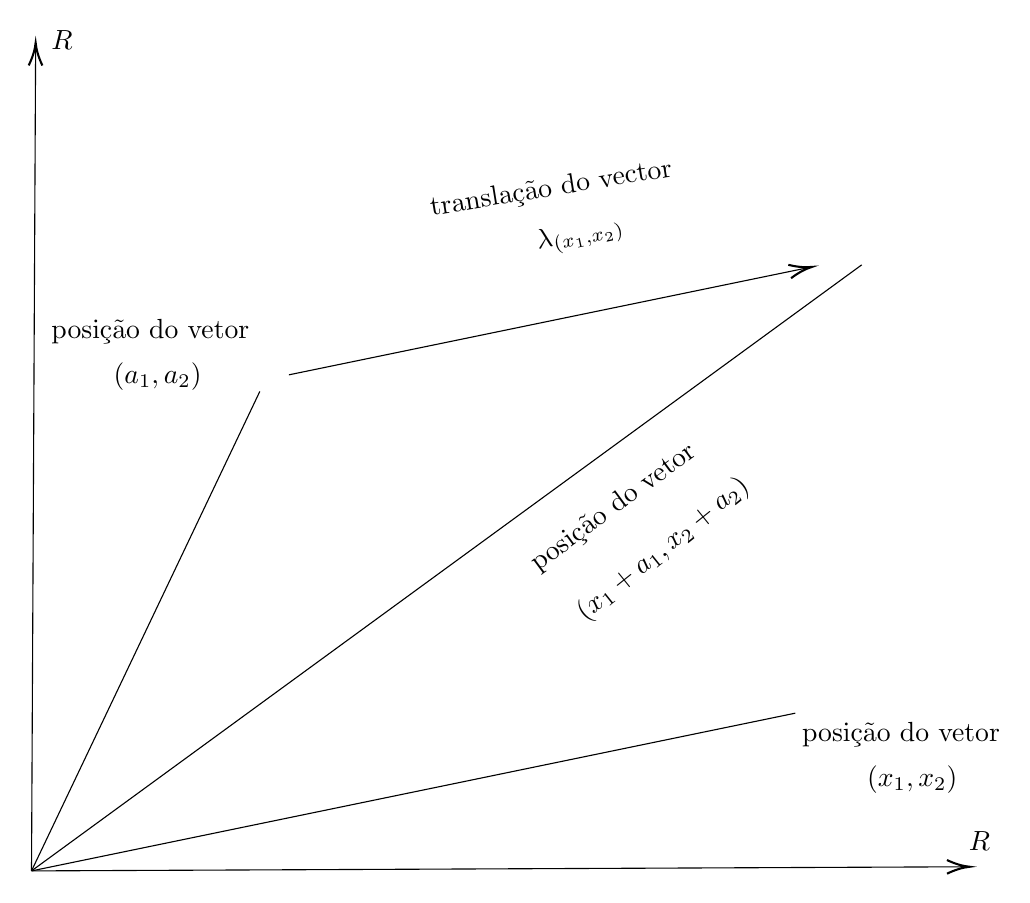
\begin{tikzpicture}[x=0.75pt,y=0.75pt,yscale=-1,xscale=1]
  %uncomment if require: \path (0,424); %set diagram left start at 0, and has height of 424
  
  %Straight Lines [id:da565732648593863] 
  \draw    (300.67,179) -- (190.67,410) ;
  %Straight Lines [id:da3637945273454497] 
  \draw    (314.67,171) -- (564.71,119.4) ;
  \draw [shift={(566.67,119)}, rotate = 168.34] [color={rgb, 255:red, 0; green, 0; blue, 0 }  ][line width=0.75]    (10.93,-3.29) .. controls (6.95,-1.4) and (3.31,-0.3) .. (0,0) .. controls (3.31,0.3) and (6.95,1.4) .. (10.93,3.29)   ;
  %Straight Lines [id:da08528271866391712] 
  \draw    (190.67,410) -- (590.67,118) ;
  %Straight Lines [id:da3340546753388143] 
  \draw    (190.67,410) -- (558.67,334) ;
  %Straight Lines [id:da119718727604893] 
  \draw    (190.67,410) -- (192.66,13) ;
  \draw [shift={(192.67,11)}, rotate = 90.29] [color={rgb, 255:red, 0; green, 0; blue, 0 }  ][line width=0.75]    (10.93,-3.29) .. controls (6.95,-1.4) and (3.31,-0.3) .. (0,0) .. controls (3.31,0.3) and (6.95,1.4) .. (10.93,3.29)   ;
  %Straight Lines [id:da7452863754317993] 
  \draw    (190.67,410) -- (640.67,408.01) ;
  \draw [shift={(642.67,408)}, rotate = 179.75] [color={rgb, 255:red, 0; green, 0; blue, 0 }  ][line width=0.75]    (10.93,-3.29) .. controls (6.95,-1.4) and (3.31,-0.3) .. (0,0) .. controls (3.31,0.3) and (6.95,1.4) .. (10.93,3.29)   ;
  
  % Text Node
  \draw (229,164) node [anchor=north west][inner sep=0.75pt]   [align=left] {$(a_{1} ,a_{2} )$};
  % Text Node
  \draw (199,143) node [anchor=north west][inner sep=0.75pt]   [align=left] {posição do vetor};
  % Text Node
  \draw (380.45,84.18) node [anchor=north west][inner sep=0.75pt]  [rotate=-350.71] [align=left] {translação do vector};
  % Text Node
  \draw (431.3,100.41) node [anchor=north west][inner sep=0.75pt]  [rotate=-347.58] [align=left] {$\lambda _{(x_{1} ,x_{2} )}$};
  % Text Node
  \draw (560.67,337) node [anchor=north west][inner sep=0.75pt]   [align=left] {posição do vetor};
  % Text Node
  \draw (592,358) node [anchor=north west][inner sep=0.75pt]   [align=left] {$(x_{1} ,x_{2} )$};
  % Text Node
  \draw (427.33,258.24) node [anchor=north west][inner sep=0.75pt]  [rotate=-323.65] [align=left] {posição do vetor};
  % Text Node
  \draw (449.31,281.74) node [anchor=north west][inner sep=0.75pt]  [rotate=-321.15] [align=left] {$(x_{1} +a_{1} ,x_{2} +a_{2} )$};
  % Text Node
  \draw (199,4) node [anchor=north west][inner sep=0.75pt]   [align=left] {$\mathbb{R}$$ $};
  % Text Node
  \draw (641,390) node [anchor=north west][inner sep=0.75pt]   [align=left] {$\mathbb{R}$$ $};   
  \end{tikzpicture}
\end{center}





